\documentclass[titlepage, 12pt]{scrartcl}

\usepackage[utf8]{inputenc}

\usepackage{amsmath,amssymb,amsthm}
\usepackage{thmtools}

\usepackage[croatian]{babel}
\usepackage{csquotes}

\usepackage[unicode]{hyperref}
\usepackage{enumitem}
\usepackage{minted}
\usepackage{graphicx}

\usepackage[style=numeric]{biblatex}
\addbibresource{literatura.bib}

\MakeOuterQuote{"}


\title{Modeliranje grafovske baze podataka za društvenu mrežu - \emph{Neo4j}}
\author{Karlo Basioli \and 
        Antonela Bogdanić \and 
        Ivan Krcivoj }
\date{Lipanj 2021}

\makeatletter         
\def\@maketitle{
\raggedright
\includegraphics[width = 40mm]{logo.jpg}\\[8ex]
\begin{center}
{\Huge \bfseries \sffamily \@title }\\[4ex] 
{\Large  \@author}\\[4ex] 
\@date\\[8ex]
\includegraphics[width = 40mm]{image.png}
\end{center}}
\makeatother

\begin{document}

\begin{titlepage}

\newcommand{\HRule}{\rule{\linewidth}{0.5mm}}
\center
\textsc{\Large Prirodoslovno-matematički fakultet}\\[1.5cm] % Name of your university/college
\textsc{\large Matematički odsjek}\\[0.5cm] % Major heading such as course name
\textsc{\large Napredne baze podataka}\\[0.5cm] 

\HRule \\[0.4cm]
{ \Large \bfseries Modeliranje grafovske baze podataka za društvenu mrežu - \emph{Neo4j}}\\[0.4cm] 
\HRule \\[1.5cm]
 

\begin{minipage}{0.4\textwidth}
\begin{flushleft} \large
\emph{Autori:}\\
Karlo \textsc{Basioli} \\
Antonela \textsc{Bogdanić} \\
Ivan \textsc{Krcivoj}
\end{flushleft}
\end{minipage}
~
\begin{minipage}{0.4\textwidth}
\begin{flushright} \large
\emph{Mentor:} \\
Ognjen \textsc{Orel} % Supervisor's Name
\end{flushright}
\end{minipage}\\[2cm]

{\large Lipanj 2021}\\[2cm] 


\includegraphics[scale=0.8]{slike/pmf_logo.jpg}\\

\vfill 

\end{titlepage}

\tableofcontents

\newpage

\section{Uvod}
Tema ovog projekta je modeliranje grafovske baze podataka za društvenu mrežu koristeći \emph{Neo4j}. Zadatak podrazumijeva odabir programskog jezika za izgradnju grafičkog sučelja, osmišljavanje i implementaciju struktura podataka potrebnih za pisanje kompleksnih upita te generiranje podataka i punjenje same baze. \\
Projekt smo u potpunosti izveli koristeći \emph{Python 3.9} programski jezik uz modul \emph{tkinter} za grafičko sučelje i modul \emph{neo4j} koji omogućava spajanje na bazu. \\
U sklopu projekta trebali smo osmisliti upit za predlaganje osoba sličnih po obrazovanju i znanju te upit za predlaganje osoba po samostalno osmišljenom kriteriju.

\newpage
\section{Struktura podataka}
Prvi problem projekta je razrada struktura podataka kojima će društvena mreža biti modelirana. Kao inspiracija poslužile su nam društvene mreže kao što su \emph{Facebook}, \emph{Twitter}, \emph{Instagram}, \emph{LinkedIn} \dots \\
Ove popularne društvene mreže danas broje stotine milijuna korisnika. Unatoč brojnim razlikama u suštini imaju sličnu poantu. Njihova zadaća je povezati korisnike. Ljudi koji koriste ove mreže mogu se međusobno dodavati za prijatelje, pratiti razne grupe, razmjenjivati poruke, dijeliti fotografije i slično. \\
Aspekt koji je gotovo uvijek zajednički je upravo spajanje korisnika. To će biti fokus ovog projekta. Trebamo osmisliti kako reprezentirati korisnika i njegove veze sa ostalim korisnicima. Također moramo ih smisleno podijeliti po edukaciji i njihovim vještinama. \\
Grafovska baza sastavljena je od vrhova koji predstavljaju osobe i fakultete u danoj bazi te relacije koje predstavljaju njihove odnose.

\subsection{Vrhovi}
\subsubsection{Person}\label{sec:Person}
Korisnik će u bazi podataka biti reprezentiran vrhom \emph{Person} sa sljedećim svojstvima:
\begin{itemize}
\begin{samepage}
    \item \textbf{id} identifikacija korisnika
    \item \textbf{name} ime korisnika
    \item \textbf{surname} prezime korisnika
    \item \textbf{gender} spol korisnika
    \item \textbf{date\_of\_birth} datum rođenja korisnika
    \item \textbf{skills} vještine koje korisnik dobija samostalno ili učenjem na fakultetu
    \item \textbf{hobbies} hobiji korisnika
\end{samepage}
\end{itemize}
Svaki \emph{id} postavljen je prilikom generiranja koda te je postavljen kao jedistven u bazi naredbom:
%TODO vidi kako ovo popraviti
\begin{samepage}
\begin{minted}[tabsize=1,breaklines]{java}
CREATE CONSTRAINT personIdConstraint ON (person:Person) ASSERT person.id IS UNIQUE;
\end{minted}
\end{samepage}
Zbog jednostavnosti prijave korisnika u aplikaciju kombinacija (\emph{name}, \emph{surname}) je jedinstvena za svakog korisnika.
\\ \\
\subsubsection{College}
Kako je važno znati edukaciju korisnika, u bazi podataka nalaziti će se i vrh \emph{College} koji predstavlja fakultet te ima sljedeća svojstva:
\begin{itemize}
\begin{samepage}
    \item \textbf{id} identifikacija korisnika
    \item \textbf{name} puno ime fakulteta
    \item \textbf{short\_name} skraćeno ime fakulteta
    \item \textbf{area} područje u koje spada fakultet
    \item \textbf{skills} vještine koje polaznik ovog fakulteta može steći
\end{samepage}
\end{itemize}
Slično kao kod vrha \emph{Person} svojstvo \textbf{id} je jedinstveno. \\
Važna pretpostavka ove baze je da je svaki njen korisnik pohađao fakultet. 
\subsection{Relacije}
\subsubsection{IS\_FRIEND}
Očito važna relacija u ovoj bazi podataka je relacija \emph{IS\_FRIEND}. Ova relacija uspostavlja se između dva vrha sa oznakom \emph{Person} i ukazuje na to da su ta dva korisnika prijatelji u ovoj društvenoj mreži. \\
Jedini atribut je:
\begin{itemize}
\begin{samepage}
    \item \textbf{start\_date} početak prijateljstva
\end{samepage}
\end{itemize}
Veza nije usmjerena te između dva korisnika postoji najviše jedna ovakva veza. \\ \\

\begin{figure}[h]
    \centering
    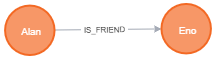
\includegraphics[scale=0.7]{slike/IS_FRIEND.png}
    \caption{Relacija \emph{IS\_FRIEND}}
    \label{fig:friendship}
\end{figure}

\subsubsection{SAME\_AREA}
Relacija \emph{SAME\_AREA} povezuje dva fakulteta koja spadaju u isto znanstveno područje. Ona služi za lakše povezivanje osoba sličnog obrazovanja. \\
Veza također nije usmjerena te dva fakulteta mogu biti povezana najviše jednom ovakvom vezom. \\
U konkretnoj bazi postoje samo tri područja.
\\ \\
\begin{figure}[h]
    \centering
    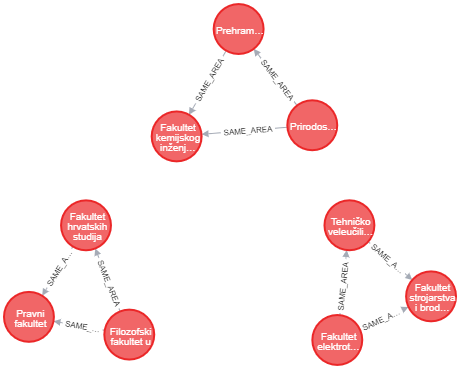
\includegraphics[scale=0.7]{slike/SAME_AREA.png}
    \caption{Relacija \emph{SAME\_AREA}}
    \label{fig:area}
\end{figure}

\subsubsection{ATTENDED}
Na kraju postoji i relacija \emph{ATTENDED}. Ovo je prva i jedina usmjerena relacija u bazi. Predstavlja vezu između korisnika i fakulteta. Ukoliko se ova dva vrha povezana bridom \emph{ATTENDED} to znači da korisnik pohađa ovaj fakultet. \\
Svojstva ove veze su:
\begin{itemize}
\begin{samepage}
    \item \textbf{enrollment\_year} godina upisa fakulteta
    \item \textbf{graduate\_year} godina završetka fakulteta
    \item \textbf{grade} prosjek ocjena dosadašnjeg studija
\end{samepage}
\end{itemize}
\begin{figure}[h]
    \centering
    
\includegraphics[scale=0.7]{slike/ATTENDED.png}
    \caption{Relacija \emph{ATTENDED}}
    \label{fig:attendance}
\end{figure}
\newpage

\section{Generiranje podataka}
Nakon što smo osmislili strukturu podataka koju ćemo koristiti bilo je potrebno stvoriti podatke kako bismo napunili našu bazu podataka. Htjeli smo da generirani podaci budu realni kako bi što bolje reprezentirali stvarni svijet. Prilikom odabira skupa podataka na temelju kojih smo generirali bazu obratili smo pozornost da ne budu previše raznoliki ali opet dovoljno bogati da bi lakše i kvalitetnije testirali upite na bazu.
\subsection{Izvori podataka}
Na internetskoj stranici \cite{imena} nalazi se popis s gotovo tisuću petsto imena kojima je pridružena oznaka spola kojem ime pripada. Popis prezimena preuzeli smo s internetske stranice \cite{prezimena}.
Kod odabira fakulteta koje će pohađati izmišljeni korisnici odlučili smo se razmatrati fakultete koji su dio Sveučilišta u Zagrebu. Kako bi podaci bili zanimljiviji odabrali smo po tri fakulteta iz tri različita područja znanosti. Područja kojima fakulteti pripadaju su:
\begin{itemize}
    \item Prirodoslovni
    \item Društveni
    \item Tehnički
\end{itemize}
Fakultete koje smo odabrali za svako područje možete vidjeti na slici \ref{fig:area}.
Za svaki fakultet napisali smo niz vještina koje osoba može steći njegovim pohađanjem.
Za kraj smo osmislili neki skup hobija kojima bi se naši korisnici mogli baviti.
\subsection{Kako su podaci generirani}
Kada smo prikupili i osmislili podatke bilo ih je potrebno pridružiti \emph{vrhovima} i \emph{bridovima}.

Imena i prezimena su na jedinstven način pridruživana osobama kako bi očuvali integritet baze.

Datum rođenja odabrali smo na slučajan način između 1980.\ i 2000.\ godine. Za taj raspon smo se odlučili kako bi svi naši korisnici bili punoljetni te mogli pohađati fakultet.

Za odabir broja hobija i vještina koje korisnik posjeduje koristili smo normalnu distribuciju.
\newpage
\begin{figure}[h]
    \centering
    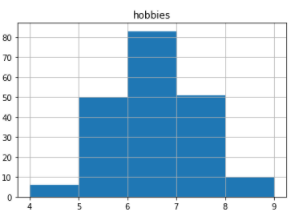
\includegraphics{slike/Hobbies_distribution.png}
    \caption{Distribucija hobija}
    \label{fig:hobbies}
\end{figure}

\begin{figure}[h]
    \centering
    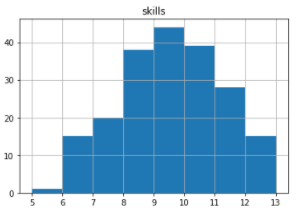
\includegraphics{slike/Skills_distribution.png}
    \caption{Distribucija vještina}
    \label{fig:skills}
\end{figure}
Kod odabira vještina pobrinuli smo se da većina vještina bude povezana s fakultetom kojeg osoba pohađa ili je pohađala a, manji broj bude ne vezan uz fakultet. Na primjer student PMF-a može biti vješt u pisanju filmskih kritika iako je to vještina koja se obično stječe na društvenim fakultetima.

Svaka osoba u prosjeku ima 10 nasumično odabranih prijatelja. Datum početka prijateljstva je nasumično odabran od trenutka kad su obje osobe napunile 18 godina do danas.

Svaka osoba pohađa ili je pohađala slučajno odabrani fakultet. Osoba je fakultet upisala nakon što je napunila 18 godina i završila ga je u roku od 5 do 10 godina. Ukoliko osoba još nije završila fakultet u \emph{graduate\_year} navodi godinu kada planira završiti fakultet.

Ocjena je decimalni broj između dva i pet zaokružen na dvije decimale. Vrijednost ocjene koju osoba ima dolazi iz normalne distribucije ali, ovisi i o broju vještina koje posjeduje. Ukoliko osoba posjeduje više vještina veće su šanse da ima bolju ocjenu.
\begin{figure}[h]
    \centering
    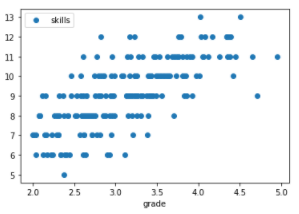
\includegraphics{slike/Grades.png}
    \caption{Ovisnost ocjene o broju vještina}
    \label{fig:hobbies}
\end{figure}

Funkcije koje stvaraju upravo opisane podatke nalaze se u datoteci \emph{db\_create.py}. 
Te funkcije stvorene podatke zapisuju u \emph{.csv} datoteke kako bi ih kasnije mogli učitati u bazu podataka.  
\newpage

\section{Implementacija aplikacije i grafičko sučelje}
Kao što je već spomenuto za izgradnju aplikacije koristili smo programski jezik \emph{Python} zbog velikog broja modula koje posjeduje i jednostavnosti korištenja tih modula. \\
Za interakciju sa bazom korišten je modul \emph{neo4j} dok se grafičko sučelje izgradilo sa modulom \emph{tkinter}.
\subsection{Modul neo4j}
Među nekoliko postojećih \emph{Python} modula za \emph{Neo4j} odabrali smo modul \emph{neo4j}. Ovaj modul podržan je od strane \emph{Neo4j} baze podataka što stoji i u dokumentaciji.\\
Za projekt je napravljena klasa \emph{Database} kao \emph{singleton} kako se ne bi nepotrebno stvarao preveliki broj različitih \emph{drivera}.

\begin{samepage}
\begin{minted}[tabsize=1,breaklines]{python}
class Database:
    __instance = None

    @staticmethod
    def get_instance(path = "database.cfg"):
        if Database.__instance == None:
            Database(path)
        return Database.__instance

    def __init__(self, path):
        if Database.__instance != None:
            raise Neo4jError("This class is a singleton!")
        else:
            #čitanje potrebnih podataka iz .cfg datoteke
            self.driver = GraphDatabase.driver(db_url, auth=(username, password))
            Database.__instance = self

    def close(self):
        self.driver.close()
\end{minted}
\end{samepage}
Prikazane su samo najosnovnije metode ove klase. \\
Instanca ove klase koristi se za slanje upita na bazu podataka. Jednostavan uzorak koji je praćen kroz cijeli projekt izgleda otprilike ovako:
\begin{samepage}
\begin{minted}[tabsize=1, breaklines]{python}
def query_database(cypher_query, args_dict, path_to_cfg):
    db = Database.get_instance(path_to_cfg)
    
    with db.driver.session() as session:
        result = session.run(cypher_query, args_dict)
    #obrada dobijenih rezultata
\end{minted}
\end{samepage}
Veliki izazov korištenja ovog modula i projekta općenito bilo je osmisliti kako puniti bazu sa generiranim podacima. Kao što je već spomenuto generirani podaci spremani su u \emph{.csv} datoteke. \\
Deklarativni jezik \emph{cypher} podržava naredbu: 
\begin{minted}{java}
LOAD CSV
\end{minted}
Ova naredba omogućava jednostavno učitavanje \emph{.csv} datoteka. Kako bi bilo omogućeno što jednostavnije punjenje baze za različite korisnike ove datoteke se pokretanjem \emph{Python} skripte šalju u \emph{import} direktorij čiji je \emph{path} potrebno zapisati u \emph{database.cfg} datoteku. \\
Upiti za učitavanje vrhova iz baze grade se na sljedeći način:
\begin{samepage}
\begin{minted}[tabsize=1,breaklines]{python}
def get_load_command_entity(self, file_name, header, entity):
    header = header.split(",")
    cypher = f"LOAD CSV WITH HEADERS FROM \"file:///{file_name}\" AS csv_line CREATE (p:{entity}" + "{"
    first = True

    for header_element in header:
        if first:
            cypher += add_attribute(header_element)
            first = False
        else:
            cypher += ", " + add_attribute(header_element)

    cypher += "});"

    return cypher
\end{minted}
\end{samepage}
Na ovaj način osigurano je jednostavno punjenje baze podataka za svakog korisnika pokretanjem skripti za generiranje podataka, a potom i skripte za punjenje baze.
\subsection{Tkinter}
\newpage

\section{Preporuke}
Postoje različiti načina stvaranja preporuka korisniku. Mnoge društvene mreže korisne razne alate i strojno učenje kako bi smislili najbolje moguće preporuke svojim korisnicima.
Neke od ovih društvenih mreža nerijetko se nalaze i u problemima s privatnosti zbog iznenađujuće preciznih preporuka.
Postoje mišljenja da ti algoritmi koriste informacije za koje korisnik nikad eksplicitno ne da dopuštenje kao što je lokacija. \\
Ovaj projekt srećom koristi generirane podatke te izbjegava probleme privatnosti. Cilj nije složiti model koji će učiti preferencije korisnika već iskoristiti grafovsku strukturu podataka kako bi po vezama između korisnika mogli dati što bolju preporuku po predodređenim kriterijima. \\
Slijede neke, možda očite, metode preporučivanja zaključno sa implementacijom naših algoritama preporučavanja.

\subsection*{Preporuke po broju zajedničkih prijatelja}
Najjednostavniji način za dobiti preporuku je poprilično izravan. Korisnik za preporuku dobija upravo one ljude s kojima ima najviše zajedničkih prijatelja. \\
U bazi \emph{neo4j} sljedećim upitom moguće je dobiti zajedničke prijatelje dva korisnika:
\begin{samepage}
\begin{minted}[tabsize=1,breaklines]{java}
MATCH (p:Person {id:72})-[i:IS_FRIEND]-(common:Person)-[j:IS_FRIEND]-
(potential_friend:Person {id: 83}) 
WHERE p.id <> potential_friend.id AND NOT ((p)-[:IS_FRIEND]-(potential_friend)) 
RETURN p, common, potential_friend,i,j;
\end{minted}
\end{samepage}
\begin{figure}[h]
    \centering
    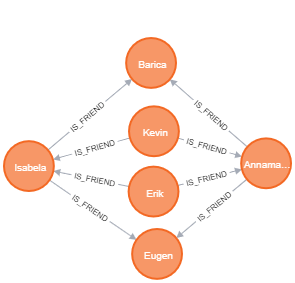
\includegraphics[scale=0.7]{slike/common_friends_query.png}
    \caption{Zajednički prijatelji}
    \label{fig:common_friends}
\end{figure}

\subsection*{Preporuke po utjecaju}
Slično kao u prethodnom primjeru i ovdje dolazi do preporuke po zajedničkim prijateljima. Ipak, u ovoj metodi situacija je nešto drugačija. \\
Pretpostavimo da imamo korisnika \emph{p} i korisnika \emph{potential\_friend} koji imaju zajedničke prijatelje, ali nisu međusobno prijatelji. \\
Pretpostavimo da su njihovi zajednički prijatelji $commons = \{c_1, c_2, \dots, c_n\}$ za koje je $friends\_num(c_i)$ jednak broju prijatelja koje korisnik $c_i$ ima. \\
Što korisnik $c_i$ ima manji broj prijatelja smatran je korisnikom koji je selektivniji u izboru svojih prijatelja. Ponekad ima smisla da veću težinu donosi selektivnija osoba zato što je izglednije da ima osobnu vezu sa korisnikom. \\
Korisniku $potential\_friend$ dodjeljuje se ocjena izračunata kao suma recipročnih vrijednosti $friends\_num(c_i)$ gdje su $c_i$ zajednički prijatelji korisnika $p$ i korisnika $potential\_friend$. \\
Formula za izračun ocjene izgleda ovako:
\begin{equation*}
    rating(potential\_friend) = \sum_{c \in commons} \frac{1}{friends\_num(c)}
\end{equation*}
Osoba sa najvećim \emph{ratingom} bit će prva preporuka po ovom algoritmu. \\
Dobro je primjetiti da je razlomak u gornjem izrazu uvijek dobro definiran pošto svaki korisnik $c$ ima barem dva prijatelja s obzirom na to da da je on zajednički prijatelj korisnicima $p$ i $potential\_friend$. \\
Slijedi upit kojim bi se izračunao \emph{rating} korisnika u \emph{cypheru}.

\begin{samepage}
\begin{minted}[tabsize=1,breaklines]{java}
MATCH (p:Person {id:72})-[:IS_FRIEND]-(common:Person)-[:IS_FRIEND]-
(potential_friend:Person {id: 83}) 
WHERE p.id <> potential_friend.id AND NOT ((p)-[:IS_FRIEND]-(potential_friend)) 
WITH common, potential_friend
MATCH (common)-[r:IS_FRIEND]-(:Person)
WITH COUNT(r) AS friends_num, common, potential_friend
RETURN SUM(1.0/friends_num) AS rating, potential_friend;
\end{minted}
\end{samepage}

\subsection*{Klasifikacijske preporuke}
Ovakav tip preporuka gleda zajednička svojstva dva korisnika i na temelju toga donosi odluku tko je kome najsličniji. \\
Za ovu bazu zajedničko svojstvo korisnika može biti fakultet koji oba korisnika pohađaju, a moguće ih je poredati po broju istih vještina koje imaju. Ovakva preporuka ima smisla zato što je logično da će se ljudi sa istog fakulteta poznavati te da je veća vjerojatnost da će se željeti sprijateljiti ako su njihove vještine slične. \\
\newpage
Primjer upita koji prikazuje sve studente na jednom fakultetu:

\begin{samepage}
\begin{minted}[tabsize=1,breaklines]{java}
MATCH (p:Person)-[att:ATTENDED]->(c:College {short_name: "TVZ"})
RETURN p, c, att LIMIT 10;
\end{minted}
\end{samepage}

Rezultat istog upita:
\begin{figure}[h]
    \centering
    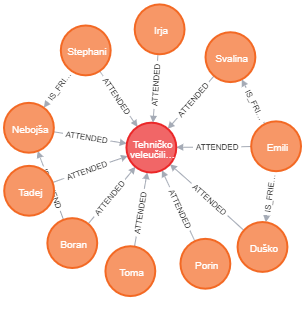
\includegraphics[scale=0.7]{slike/same_college.png}
    \caption{Studenti \emph{TVZ}-a}
    \label{fig:common_friends}
\end{figure}

Ovo su neke od metoda koje se mogu koristiti za preporuke u društvenim mrežama te su poslužile kao inspiracija za upite kojima aplikacija predlaže korisnicima njihove potencijalne prijatelje. \\
Dio projekta bio je osmisliti upite koji će predlagati prijatelje na temelju znanja i obrazovanja te za osobne preporuke.

\subsection{Poslovne preporuke}
Želja je omogućiti korisniku brzo i efikasno umrežavanje sa ljudima istih ili sličnih vještina. \\
Izglednije je da će korisnik dodati osobu sličnih vještina zbog mogućnosti suradnje. Ovo podosta zvuči kao klasifikacijska preporuka, no je li moguće dodatno personalizirati preporuke na temelju postojećih informacija? \\
Očito je korisniku važno upoznati ljude sa srodnih fakulteta. To će biti prvi filter preporuka.\\
Upit je prezentiran u koracima. \\
U idućem upitu primjetite nizove znakova nakon dolara. To su vrijednosti koje korisnik predaje prilikom slanja upita. Ako je aplikaciju uključila osoba sa identifikacijskim brojem $14$ tada će se idući upit izvršiti s tim identifikacijskim brojem.

\begin{samepage}
\begin{minted}[tabsize=1,breaklines]{java}
MATCH (p:Person {id:$id})-[:ATTENDED]->(:College)-[:SAME_AREA]-
(:College)<-[:ATTENDED]-(recommendation:Person)
WHERE p.id <> recommendation.id AND NOT((p)-[:IS_FRIEND]-(recommendation))

\end{minted}
\end{samepage}
Idući dio ovisi o korisniku. Ljudi različitog godišta imaju različite poslovne interese. \\
Mlađi ljudi će zbog srama, neiskustva i sličnog teže pristupiti  iskusnijoj osobi. Izglednije je da će mlađa osoba htjeti dodati svoje vršnjake koji imaju slična iskustva. \\
S druge strane iskusnija osoba mari manje za to i više ju zanimaju vještine korisnika. Na primjer poslodavcu može biti zanimljivo zaposliti studenta kao ulaganje u budućnost, ali može mu od interesa biti i zapošljavanje iskusnih ljudi iz njegovog područja. \\
Dakle idući filter za mlade ljude bit će razlika u godinama, što je manja izglednije je da će joj se ta osoba preporučiti dok će za starije ljude filter biti presjek istih vještina koje osoba ima. \\
Sada kada su preporuke dodatno sužene, ako je to potrebno, opet po godištu dodajemo nove filtere. \\
U ovom slučaju ćemo zamijeniti uloge. Mlađi ljudi će sada u svojem popisu preporuka imati ljude sličnog godišta pa će se te preporuke filtrirati po presjeku vještina zato što je izglednije da će mladi ljudi htjeti dodati osobu zainteresiranu za njihovo područje. \\
Starijim korisnicima filter će djelovati suprotno od filtera za mlađe korisnike. Preporuke će poredati po razlici u godinama kako bi im predstavili najiskusnije ljude iz njihovog područja. \\
Slijedi nastavak na prethodni komad koda sastavljen od navedena dva filtera za starije korisnike:
\begin{samepage}
\begin{minted}[tabsize=1,breaklines]{java}
WITH p, recommendation, size([x IN p.skills WHERE x IN recommendation.skills]) AS common_skills 
ORDER BY common_skills DESC LIMIT $first_limit
RETURN recommendation, abs(p.date_of_birth.year - recommendation.date_of_birth.year) AS birth_delta 
ORDER BY birth_delta DESC LIMIT $limit;

\end{minted}
\end{samepage}
\newpage
Rezultat sljedećeg upita za korisnicu Lori Vulin vidljiv je na grafičkom sučelju:

\begin{figure}[h]
    \centering
    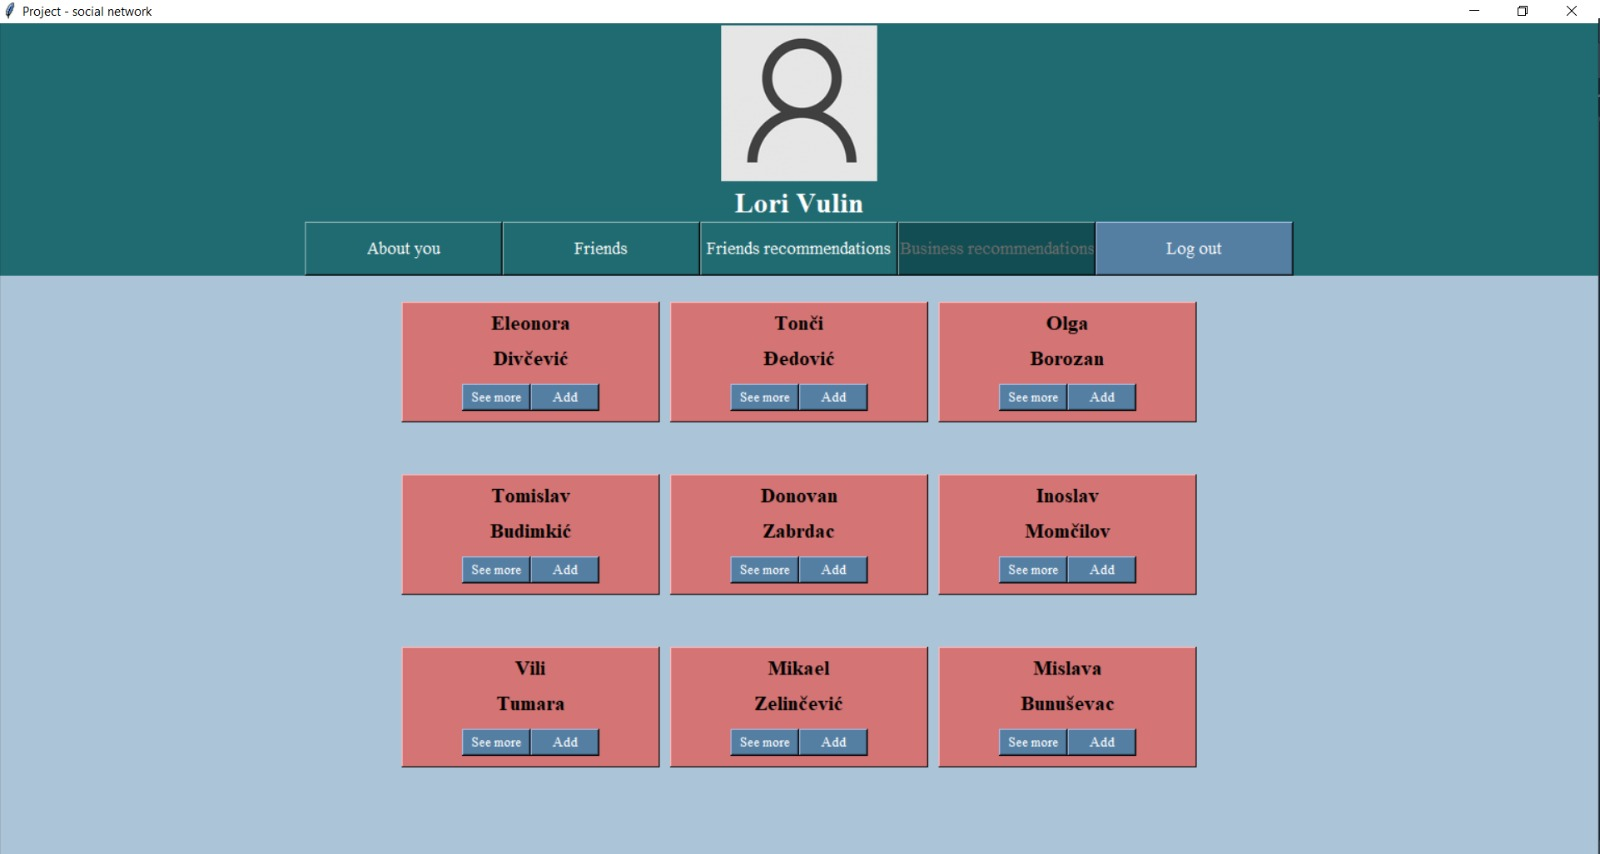
\includegraphics[scale=0.19]{slike/business.jpg}
    \caption{Poslovne preporuke}
    \label{fig:business_rec}
\end{figure}

\subsection{Osobne preporuke}
Slično kao poslovne preporuke osobne preporuke se odvijaju u nekoliko koraka. \\
Prvi korak je odabir osoba sa najviše zajedničkih prijatelja kako bi postojala veća vjerojatnost poznanstva.
\begin{samepage}
\begin{minted}[tabsize=1,breaklines]{java}
MATCH (p:Person {id:$id})-[:IS_FRIEND]-(:Person)-[:IS_FRIEND]-(recommendation:Person)
WHERE p.id <> recommendation.id AND NOT((p)-[:IS_FRIEND]-(recommendation))
WITH p, recommendation, count(recommendation) AS common_friends
ORDER BY common_friends DESC LIMIT $first_limit

\end{minted}
\end{samepage}
Ovoga puta je drugi korak za sve isti. Ljudi se češće druže sa ljudima svojeg godišta pa idući filter odabire najbliže ljude po godištu:
\begin{samepage}
\begin{minted}[tabsize=1,breaklines]{java}
WITH p, recommendation, abs(recommendation.date_of_birth.year - p.date_of_birth.year) AS birth_delta 
ORDER BY birth_delta LIMIT $second_limit

\end{minted}
\end{samepage}

Finalno potrebno je provjeriti kombatibilnost korisnika. Sada je osim presjeka vještina u obzir uzet i presjek hobija. \\
Očito može biti važno da ljudi imaju iste vještine s obzirom da iz toga često proizlaze poznanstva, ali istom logikom važan je i presjek hobija. \\
Ako se dvoje ljudi bavi istom aktivnosti u slobodno vrijeme izgledno je da bi se mogli slagati ili se već poznaju. \\
Ovime se finalizira upit koji za osobne preporuke ljudima:
\begin{samepage}
\begin{minted}[tabsize=1,breaklines]{java}
RETURN recommendation, size([skill IN p.skills WHERE skill IN recommendation.skills]) + size([hobby IN p.hobbies WHERE hobby IN recommendation.hobbies]) AS common 
ORDER BY common DESC LIMIT $limit;

\end{minted}
\end{samepage}
\newpage
\begin{samepage}
Rezultate upita moguće je vidjeti na grafičkom sučelju:
\begin{figure}[h]
    \centering
    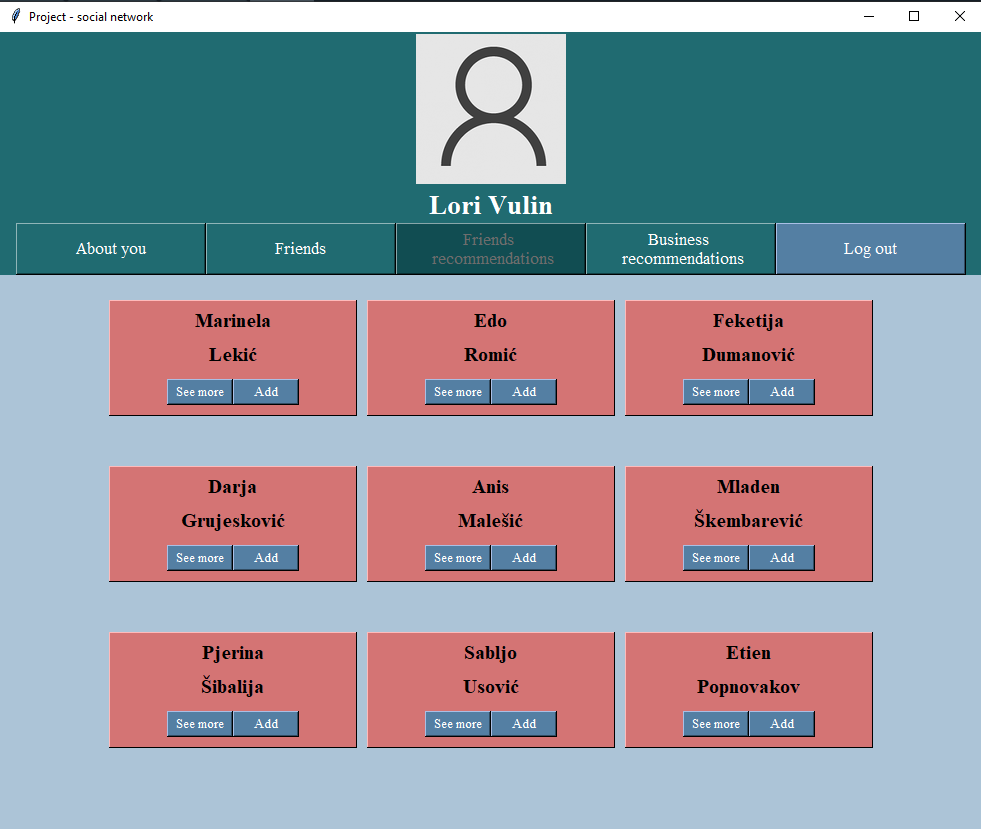
\includegraphics[scale=0.19]{slike/personal.jpg}
    \caption{Osobne preporuke}
    \label{fig:personal_rec}
\end{figure}
\end{samepage}

\subsection{Brzina izvršavanja upita}
Zanimljiva stvar koja je uočena prilikom stvaranja aplikacije je neovisnost trajanja upita o veličini baze. Odabrani su najsloženiji upiti, što su upravo upiti za preporučavanje prijatelja te se \emph{Pythonovom} bibliotekom \emph{time} mjerilo vrijeme izvršavanja svakog upita. \\
Napravljeno je po deset baza za svaku od veličina iz skupa $\{50, 100, 150, \dots, 1000\}$ gdje elementi skupa predstavljaju broj osoba koji se nalaze u bazi podataka. Za svaku od tih baza upit je poslan za tri nasumično odabrana korisnika te su dobijeni sljedeći rezultati.\\

\begin{figure}[h]
    \centering
    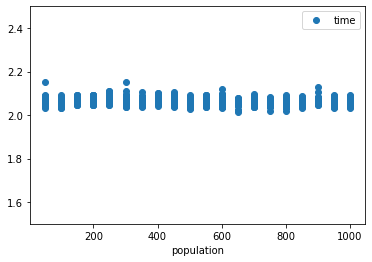
\includegraphics[scale=0.5]{slike/personal_graph.png}
    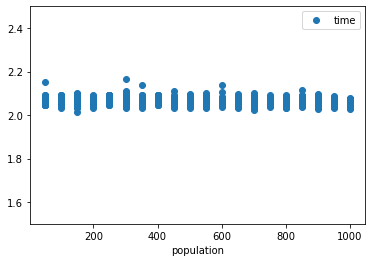
\includegraphics[scale=0.5]{slike/business_graph.png}
    \caption{Brzina upita}
    \label{fig:query_speed}
\end{figure}


Iznenađujuće vrijeme izvršavanja upita ostaje konstantno te traje nešto više od dvije sekunde. \\
Iako na prvu ruku rezultat izgleda neočekivano razlog u tome nalazimo na naviku korištenja relacijskih baza podataka gdje bi za većinu ovakvih upita bilo potrebno raditi Kartezijev produkt tablica za što je prirodno očekivati da će rastom veličine tablice trebati puno više vremena. \\
Međutim ovdje ne dolazi do Kartezijevog produkta već se pretraživanje odvija grafovskim algoritmima što daje veliko ubrzanje 


\newpage
\section{Zaključak}

\end{document}
